%%%%%%%%%%%%%%%%%%%%%%%%%%%%%%%%%%%%%%%%%
% a0poster Landscape Poster
% LaTeX Template
% Version 1.0 (22/06/13)
%
% The a0poster class was created by:
% Gerlinde Kettl and Matthias Weiser (tex@kettl.de)
%
% This template has been downloaded from:
% http://www.LaTeXTemplates.com
%
% License:
% CC BY-NC-SA 3.0 (http://creativecommons.org/licenses/by-nc-sa/3.0/)
%
%%%%%%%%%%%%%%%%%%%%%%%%%%%%%%%%%%%%%%%%%

%----------------------------------------------------------------------------------------
%	PACKAGES AND OTHER DOCUMENT CONFIGURATIONS
%----------------------------------------------------------------------------------------

\documentclass[a0,landscape]{a0poster}

\usepackage{multicol} % This is so we can have multiple columns of text side-by-side
\columnsep=80pt % This is the amount of white space between the columns in the poster
\columnseprule=3pt % This is the thickness of the black line between the columns in the poster

\usepackage[svgnames]{xcolor} % Specify colors by their 'svgnames', for a full list of all colors available see here: http://www.latextemplates.com/svgnames-colors

\usepackage{times} % Use the times font
%\usepackage{palatino} % Uncomment to use the Palatino font

\usepackage{graphicx} % Required for including images
\graphicspath{{figures/}} % Location of the graphics files
\usepackage{booktabs} % Top and bottom rules for table
\usepackage[font=small,labelfont=bf]{caption} % Required for specifying captions to tables and figures
\usepackage{amsfonts, amsmath, amsthm, amssymb} % For math fonts, symbols and environments
\usepackage{wrapfig} % Allows wrapping text around tables and figures
\usepackage[utf8]{inputenc} % Pour utiliser les caractères accentués
\usepackage{tikz}
\begin{document}

%----------------------------------------------------------------------------------------
%	POSTER HEADER
%----------------------------------------------------------------------------------------

% The header is divided into three boxes:
% The first is 55% wide and houses the title, subtitle, names and university/organization
% The second is 25% wide and houses contact information
% The third is 19% wide and houses a logo for your university/organization or a photo of you
% The widths of these boxes can be easily edited to accommodate your content as you see fit

\noindent\begin{minipage}[b]{\linewidth}
\centering
\noindent \veryHuge \color{NavyBlue} \textbf{Lake-river and lake-atmosphere interactions in a changing climate over Northeast Canada} \color{Black}\\ % Title
\noindent\begin{minipage}[c]{0.2\linewidth}
      \center
      
\includegraphics[width=25cm]{logo_cnrcwp_escer.png} % Logo or a photo of you, adjust its dimensions here
\end{minipage} \hfill
%
\begin{minipage}[c]{0.15\linewidth}
  \center
  \Large \textbf{Oleksandr Huziy} \\
  \large \texttt{guziy.sasha@gmail.com}
\end{minipage}
%
\begin{minipage}[b]{0.01\linewidth}
 \center
 \Large\&
\end{minipage}
%
\begin{minipage}[c]{0.15\linewidth}
   \center
   \Large \textbf{Laxmi Sushama} \\
   \large  \texttt{sushama.laxmi@uqam.ca}
\end{minipage}\hfill
%
\begin{minipage}[c]{0.2\linewidth}
  \center
  
\includegraphics[width=15cm]{logo_uqam.png} % Logo or a photo of you, adjust its dimensions here
\end{minipage}
\rule{\linewidth}{3pt}
\end{minipage}
%

\vspace{0.5cm} % A bit of extra whitespace between the header and poster content

%----------------------------------------------------------------------------------------

\begin{multicols}{3} % This is how many columns your poster will be broken into, a poster with many figures may benefit from less columns whereas a text-heavy poster benefits from more

%----------------------------------------------------------------------------------------
%	ABSTRACT
%----------------------------------------------------------------------------------------

\color{Navy} % Navy color for the abstract

\begin{abstract}
Lakes influence the regional climate and hydrology in a number of ways and therefore they should be represented
in climate models in a realistic manner. Lack of representation of lakes in models can lead to errors in simulated
energy and water fluxes, for lake-rich regions. This study focuses on the assessment of the impact of climate
change on lakes and hydrology as well as on the influence of lakes on projected changes to regional climate
and surface hydrology, particularly streamflows, for Northeast Canada. To this end, transient climate change
simulations spanning the 1950–2100 period are performed, with and without lakes, with the fifth generation of
the Canadian Regional Climate Model (CRCM5), driven by the Canadian Earth System Model (CanESM2) at the
lateral boundaries for Representative Concentration Pathway 8.5.

Comparison of projected changes from the CRCM5 simulations with and without lakes suggest that lakes
attenuate projected increases to 2-m air temperature in all seasons, almost everywhere in the study domain, with
maximum decreases of the order of 2$^\circ$C occurring during winter. As for streamflows, results suggest projected
increases for winter and spring and decreases during summer. Comparison of the projected changes suggests
that lakes attenuate the projected increases in streamflows in spring due to the storage effect of lakes, and
also attenuate the projected decreases in streamflows in summer in future climate due to the gradual release of
the excess water stored in the lakes during spring. This study, thus demonstrates the impact of lakes on projected
changes to the regional climate and hydrology for the study region using a single regional modelling system.
\end{abstract}

%----------------------------------------------------------------------------------------
%	INTRODUCTION
%----------------------------------------------------------------------------------------

\color{SaddleBrown} % SaddleBrown color for the introduction

\section*{(A) Introduction}
Inland water bodies, such as lakes and rivers, are essential for human
livelihood (i.e. drinking water, agriculture, hydroelectricity, transportation),
and this has led to many activities around lakes and rivers, which in turn
resulted in the development of expensive and important infrastructure in the
proximity of such water bodies. The safety and proper functioning of these
infrastructures in the context of a changing climate is a major concern. For
this reason, it is important to assess projected changes to the hydrological
cycle and related uncertainties.

Though many climate models, particularly RCMs, include lakes, only few studies
have attempted to realistically simulate the water balance of lakes, considering
inflows and outflows of lakes, and the impact of lakes on streamflows. Huziy and
Sushama (2015) recently implemented a river/lake routing scheme, interflow
process, i.e. the lateral flow of water in the top soil layers along topographic
slopes, and interactions between lakes and rivers in terms of water balance in
the fifth generation Canadian Regional Climate Model (CRCM5). By including lake
routing, they noticed significant improvements to the simulated spring peak and
winter low flows, which were too high and too low, respectively, without the
lake-river interaction. The impacts of interflow on simulated streamflow and on
the regional climate were modest according to their study. These new
implementations in CRCM5 by Huziy and Sushama (2015) resulted in a more
comprehensive tool for regional climate change studies that can be used to
better understand interactions between atmosphere, lakes and rivers in the
context of a changing climate.

This study therefore focuses on the projected changes to the regional climate
and hydrology for northeastern Canada using CRCM5, and estimates the
impacts of lake-river, lake-atmosphere interactions and of interflow on the
projected changes to selected hydrologic/near-surface climate variables under
the Representative Concentration Pathway 8.5 (RCP85). For this scenario, the
concentration of greenhouse gases in the atmosphere continues to rise during the
21st century, causing an increase in the radiative forcing of 8.5 ${\rm W/m^2}$ by 2100
with respect to the preindustrial period. The study domain covers 21
watersheds that are important for various economic activities (notably
hydropower generation) and contain a large number of subgrid lakes for which the
use of a 1D column lake model is appropriate.

%----------------------------------------------------------------------------------------
%	OBJECTIVES
%----------------------------------------------------------------------------------------

\color{DarkSlateGray} % DarkSlateGray color for the rest of the content

\section*{(B) Main Objectives}

\begin{enumerate}
\item Improve most important processes essential for simulating streamflow (rivers, river-lake connectivity, etc).
\item Study/quantify atm.-lake-river interactions through carefully designed experiments.
\item Study/quantify impact of lake-atmosphere, of lake-river interactions on the projected changes to selected hydrological/near-surface climate variables over northeastern Canada.
\end{enumerate}

%----------------------------------------------------------------------------------------
%	MATERIALS AND METHODS
%----------------------------------------------------------------------------------------

\section*{(C) Methods and experiment configurations}
\subsection*{(C.1) Methods}
The impacts of lake-atmosphere interactions on
projected changes and the impacts of direct lake-river interactions on projected
changes in streamflow are assessed using the configurations with and without
lakes, described below.

%
\begin{minipage}[t]{\linewidth}
\center
\small
\begin{tabular}{lll}
\toprule
\textbf{Simulation} & \textbf{Period} & \textbf{Description}\\
\midrule
ERAI-CRCM5-L     & 1979--2010 & Reanalysis-driven, includes lake-atm. and lake-river interactions\\
CanESM2-CRCM5-NL & 1950--2100 & CanESM2-driven, lakes are replaced with bare ground \\
CanESM2-CRCM5-L  & 1950--2100 & CanESM2-driven, includes lake-atm. and lake-river interactions \\
\bottomrule
\end{tabular}
\captionof{table}{\color{Green} List of simulations used in the current study}
\end{minipage}

%
\begin{minipage}[t]{\linewidth}
\begin{tikzpicture}
    % schematics
    \node[label={\small NL (no lakes)}] (nl) at (0,0) {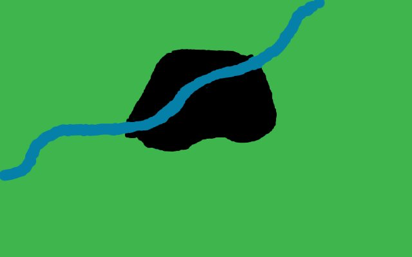
\includegraphics[scale=0.5]{crcm5-nl}};
    \node[label={\small L (with lakes)}] (wl) at (0,-5) {
\includegraphics[scale=0.5]{crcm5-l}};

    \node (middle) at (6, -2.5) {


    };

    % lines
    \draw[line width=5pt] (nl.east) -- (middle.west);
    \draw[line width=5pt] (wl.east) -- (middle.west);

    % explanation bullets
    \node[text width=\linewidth, align=left] (b1) at (8, -1) {$\bullet$ By comparing projected changes to atmospheric fields $\longrightarrow$ Impact of lake-atm. interactions.};
    \node[text width=\linewidth, align=left] (b2) at (8, -4) {$\bullet$ By comparing projected changes to streamflow $\longrightarrow$ Direct \& indirect impact of lakes on rivers.};

\end{tikzpicture}
\end{minipage}




\subsection*{(C.2) Experiment setup}
  \begin{minipage}[b]{0.5\linewidth}
    \center
    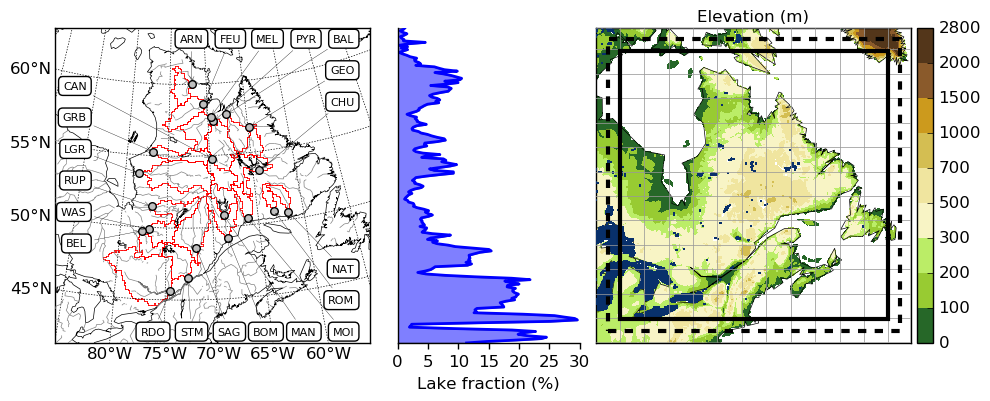
\includegraphics[width=\linewidth]{qc_basin_outlets_points}
    \captionof{figure}{\color{Green} Left panel: domain with basins of interest, the grey circles show basin outlets determined from the flow
    direction field, used for streamflow simulations; middle panel: zonally averaged lake fractions. Right panel: topography [m], the cells with lake fractions greater or equal to 0.6 are indicated with blue colour,
    the gray cells contain 20$\times$20 grid cells.}
  \end{minipage} \hfill
%
\begin{minipage}[b]{0.45\linewidth}
\flushleft
\begin{itemize}
  \item Horizontal grid: 260$\times$260, \color{Red} dx=0.1$^\circ$ \color{DarkSlateGray};
  \item Time step: \color{Red} 5 min \color{DarkSlateGray};
  \item Simulation periods:\\ \textbf{1979--2010} (current climate, validation), \textbf{1950--2100} (climate change);
  \item Analysis periods:\\ \textbf{1980--2010} (current), \textbf{2070--2100} (future);
  \item Surface scheme: CLASS3.5;
  \item Lake model: Hostetler;
  \item River model: WATROUTE-modified;
  \item Lateral boundary conditions:
    \begin{itemize}
        \item ERA-Interim, 1.5$^\circ$
        \item CanESM2 outputs
    \end{itemize}

\end{itemize}
\end{minipage}

%----------------------------------------------------------------------------------------
%	RESULTS
%----------------------------------------------------------------------------------------

\section*{(D) Results}

\subsection*{(D.1) Validation}
\begin{minipage}[t]{0.45\linewidth}
\begin{center}
  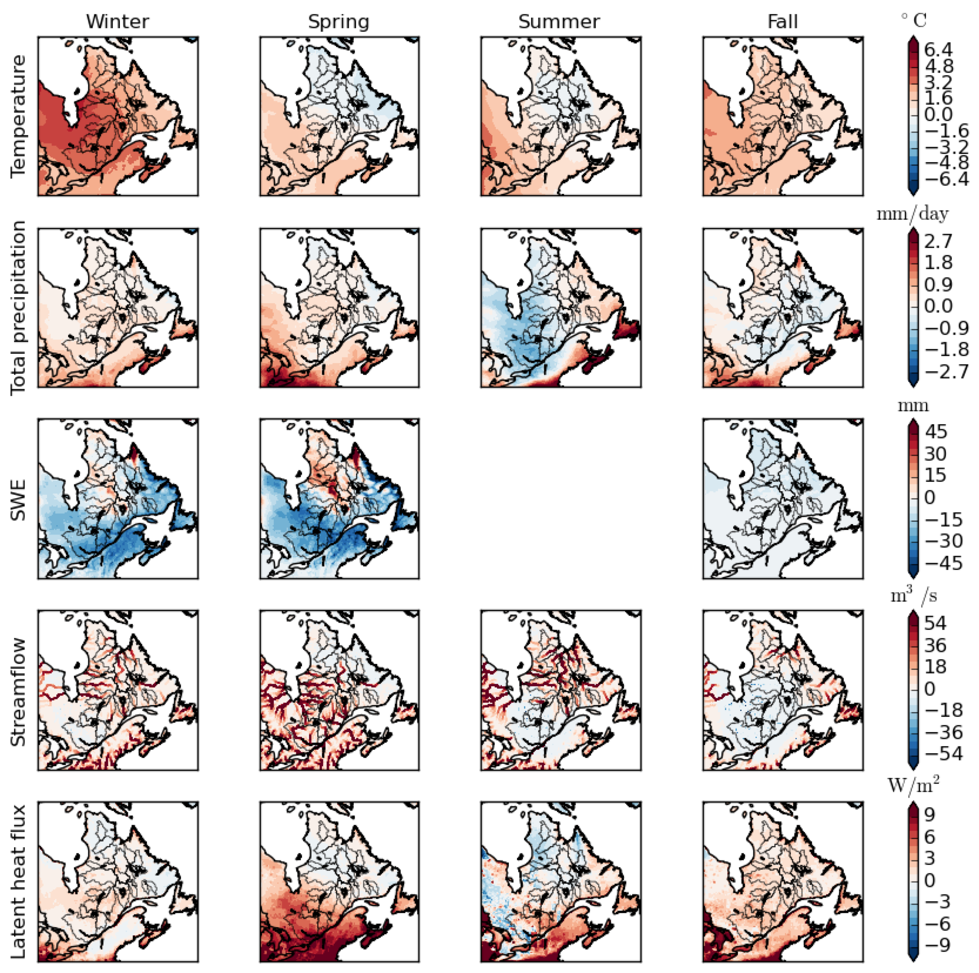
\includegraphics[width=\linewidth]{bfe_atm}
  \captionof{figure}{\color{Green} Boundary forcing errors, i.e. differences between CanESM2-CRCM5-L and ERAI- CRCM5-L simulations for the 1980–2010 period, for 2-m air temperature [$^\circ$C] (first row), total precipitation [mm/day] (second row), SWE [mm] (third row) and streamflows [m$^3$/s] (fourth row).}
\end{center}
\end{minipage}\hfill
%
\begin{minipage}[t]{0.45\linewidth}
\begin{center}
  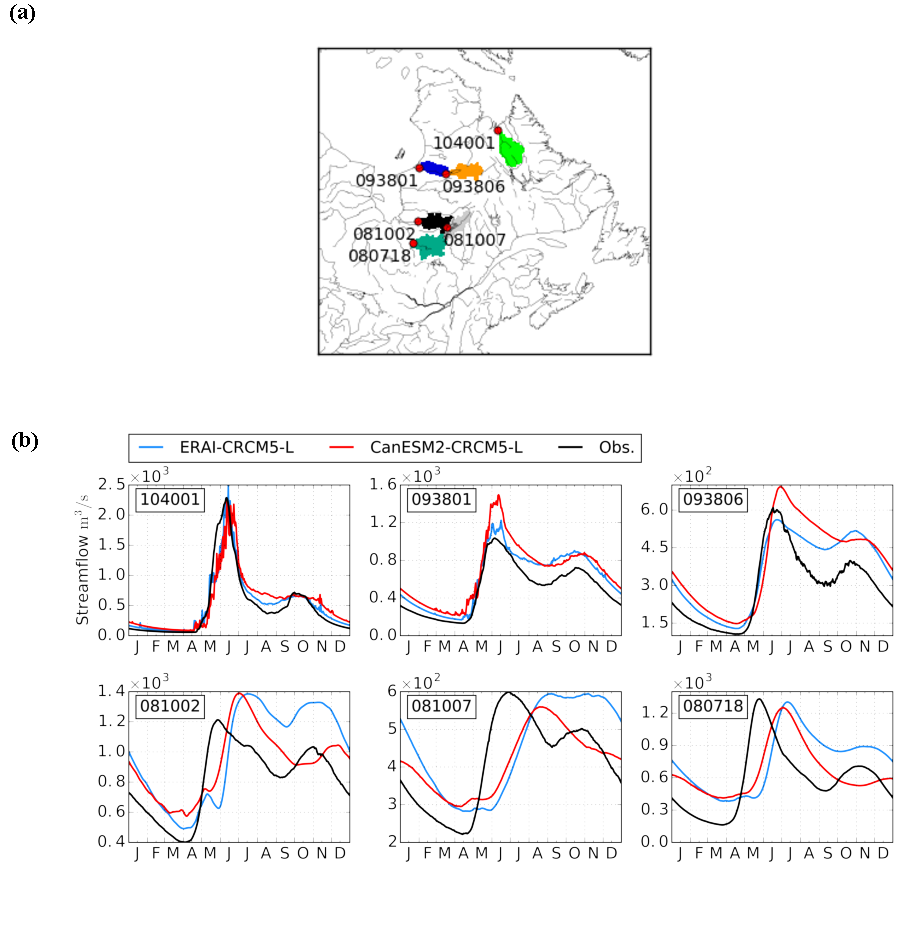
\includegraphics[width=\linewidth]{streamflow_validation_6}
  \captionof{figure}{\color{Green} (a) Locations and identification numbers (IDs) of the selected gauging stations with their upstream areas (determined from the flow directions field) shown shaded. (b) Comparison of observed (black) and modelled (blue and red correspond to ERAI-CRCM5-L and CanESM2-CRCM5-L simulations, respectively) daily climatological streamflow [m3/s] at selected stations. }
\end{center}
\end{minipage}
%

\subsection*{(D.2) Impacts of lake-atmosphere and lake-river interactions on projected climate changes}




Phasellus imperdiet, tortor vitae congue bibendum, felis enim sagittis lorem, et volutpat ante orci sagittis mi. Morbi rutrum laoreet semper. Morbi accumsan enim nec tortor consectetur non commodo nisi sollicitudin. Proin sollicitudin. Pellentesque eget orci eros. Fusce ultricies, tellus et pellentesque fringilla, ante massa luctus libero, quis tristique purus urna nec nibh.

Nulla ut porttitor enim. Suspendisse venenatis dui eget eros gravida tempor. Mauris feugiat elit et augue placerat ultrices. Morbi accumsan enim nec tortor consectetur non commodo. Pellentesque condimentum dui. Etiam sagittis purus non tellus tempor volutpat. Donec et dui non massa tristique adipiscing. Quisque vestibulum eros eu. Phasellus imperdiet, tortor vitae congue bibendum, felis enim sagittis lorem, et volutpat ante orci sagittis mi. Morbi rutrum laoreet semper. Morbi accumsan enim nec tortor consectetur non commodo nisi sollicitudin.

\begin{center}\vspace{1cm}

\includegraphics[width=0.8\linewidth]{placeholder}
\captionof{figure}{\color{Green} Figure caption}
\end{center}\vspace{1cm}

In hac habitasse platea dictumst. Etiam placerat, risus ac.

Adipiscing lectus in magna blandit:

\begin{center}\vspace{1cm}
\begin{tabular}{l l l l}
\toprule
\textbf{Treatments} & \textbf{Response 1} & \textbf{Response 2} \\
\midrule
Treatment 1 & 0.0003262 & 0.562 \\
Treatment 2 & 0.0015681 & 0.910 \\
Treatment 3 & 0.0009271 & 0.296 \\
\bottomrule
\end{tabular}
\captionof{table}{\color{Green} Table caption}
\end{center}\vspace{1cm}

Vivamus sed nibh ac metus tristique tristique a vitae ante. Sed lobortis mi ut arcu fringilla et adipiscing ligula rutrum. Aenean turpis velit, placerat eget tincidunt nec, ornare in nisl. In placerat.

\begin{center}\vspace{1cm}

\includegraphics[width=0.8\linewidth]{placeholder}
\captionof{figure}{\color{Green} Figure caption}
\end{center}\vspace{1cm}

%----------------------------------------------------------------------------------------
%	CONCLUSIONS
%----------------------------------------------------------------------------------------

\color{SaddleBrown} % SaddleBrown color for the conclusions to make them stand out

\section*{(E) Conclusions}

\begin{itemize}
\item Comparison of projected changes from the simulations with and without lakes suggests important impact of lakes on projected increases to 2-m temperatures, due to thermal inertia of lakes.
\item Amplitudes of projected changes to streamflows are mostly dampened by lake-river interactions. Although a north-south dipole pattern, due to frozen conditions, can be noted in winter.
\end{itemize}

\color{DarkSlateGray} % Set the color back to DarkSlateGray for the rest of the content


 %----------------------------------------------------------------------------------------
%	REFERENCES
%----------------------------------------------------------------------------------------

\nocite{*} % Print all references regardless of whether they were cited in the poster or not
\bibliographystyle{plain} % Plain referencing style
\bibliography{sample} % Use the example bibliography file sample.bib

%----------------------------------------------------------------------------------------
%	ACKNOWLEDGEMENTS
%----------------------------------------------------------------------------------------

\section*{Acknowledgements}
This research was carried out within the Canadian Network for Regional Climate and Weather Processes (CNRCWP) project funded by the Natural Sciences and Engineering Research Council (NSERC) of Canada.
%----------------------------------------------------------------------------------------

\end{multicols}
\end{document}
